% Options for packages loaded elsewhere
\PassOptionsToPackage{unicode,pdfpagelabels}{hyperref}
\PassOptionsToPackage{hyphens}{url}
\PassOptionsToPackage{dvipsnames,svgnames,x11names}{xcolor}
%
\documentclass[
  12pt,
  a4paper,
]{report}

\usepackage{amsmath,amssymb}
\usepackage{iftex}
\ifPDFTeX
  \usepackage[T1]{fontenc}
  \usepackage[utf8]{inputenc}
  \usepackage{textcomp} % provide euro and other symbols
\else % if luatex or xetex
  \usepackage{unicode-math}
  \defaultfontfeatures{Scale=MatchLowercase}
  \defaultfontfeatures[\rmfamily]{Ligatures=TeX,Scale=1}
\fi
\usepackage[]{lmodern}
\ifPDFTeX\else  
    % xetex/luatex font selection
\fi
% Use upquote if available, for straight quotes in verbatim environments
\IfFileExists{upquote.sty}{\usepackage{upquote}}{}
\IfFileExists{microtype.sty}{% use microtype if available
  \usepackage[]{microtype}
  \UseMicrotypeSet[protrusion]{basicmath} % disable protrusion for tt fonts
}{}
\makeatletter
\@ifundefined{KOMAClassName}{% if non-KOMA class
  \IfFileExists{parskip.sty}{%
    \usepackage{parskip}
  }{% else
    \setlength{\parindent}{0pt}
    \setlength{\parskip}{6pt plus 2pt minus 1pt}}
}{% if KOMA class
  \KOMAoptions{parskip=half}}
\makeatother
\usepackage{xcolor}
\usepackage[top=2cm,bottom=2cm,left=1.5cm,right=1.5cm,marginparsep=2cm]{geometry}
\setlength{\emergencystretch}{3em} % prevent overfull lines
\setcounter{secnumdepth}{5}
% Make \paragraph and \subparagraph free-standing
\makeatletter
\ifx\paragraph\undefined\else
  \let\oldparagraph\paragraph
  \renewcommand{\paragraph}{
    \@ifstar
      \xxxParagraphStar
      \xxxParagraphNoStar
  }
  \newcommand{\xxxParagraphStar}[1]{\oldparagraph*{#1}\mbox{}}
  \newcommand{\xxxParagraphNoStar}[1]{\oldparagraph{#1}\mbox{}}
\fi
\ifx\subparagraph\undefined\else
  \let\oldsubparagraph\subparagraph
  \renewcommand{\subparagraph}{
    \@ifstar
      \xxxSubParagraphStar
      \xxxSubParagraphNoStar
  }
  \newcommand{\xxxSubParagraphStar}[1]{\oldsubparagraph*{#1}\mbox{}}
  \newcommand{\xxxSubParagraphNoStar}[1]{\oldsubparagraph{#1}\mbox{}}
\fi
\makeatother


\providecommand{\tightlist}{%
  \setlength{\itemsep}{0pt}\setlength{\parskip}{0pt}}\usepackage{longtable,booktabs,array}
\usepackage{calc} % for calculating minipage widths
% Correct order of tables after \paragraph or \subparagraph
\usepackage{etoolbox}
\makeatletter
\patchcmd\longtable{\par}{\if@noskipsec\mbox{}\fi\par}{}{}
\makeatother
% Allow footnotes in longtable head/foot
\IfFileExists{footnotehyper.sty}{\usepackage{footnotehyper}}{\usepackage{footnote}}
\makesavenoteenv{longtable}
\usepackage{graphicx}
\makeatletter
\def\maxwidth{\ifdim\Gin@nat@width>\linewidth\linewidth\else\Gin@nat@width\fi}
\def\maxheight{\ifdim\Gin@nat@height>\textheight\textheight\else\Gin@nat@height\fi}
\makeatother
% Scale images if necessary, so that they will not overflow the page
% margins by default, and it is still possible to overwrite the defaults
% using explicit options in \includegraphics[width, height, ...]{}
\setkeys{Gin}{width=\maxwidth,height=\maxheight,keepaspectratio}
% Set default figure placement to htbp
\makeatletter
\def\fps@figure{htbp}
\makeatother

\usepackage{geometry}       % Control page margins
\usepackage{setspace}       % Custom line spacing
\usepackage{titlesec}       % Modern section titles
\usepackage{amsmath}        % Math environments
\usepackage{amssymb}        % Math symbols
\usepackage{amsfonts}       % Math fonts
\usepackage{mathtools}      % Extra math tools
\usepackage{physics}        % For partial derivatives
\usepackage{siunitx}        % SI units
\sisetup{per-mode = symbol} % Set SI unit fractions to use a solidus
\usepackage{commath}        % For derivatives

\usepackage{graphicx}       % For including images
\usepackage{xcolor}         % Color text, if needed
\usepackage{xparse}
\usepackage{booktabs}       % Improved tables
\usepackage{enumitem}       % Customized lists
\usepackage{float}          % Improved figure placement
\usepackage{tikz}           % Core TikZ package
\usetikzlibrary{positioning, arrows.meta}
\usepackage{circuitikz}     % For circuits!
\usepackage{pgfplots}       % For plots
\pgfplotsset{compat=1.18}   % Set compatibility to 1.18
\usepackage{fancyhdr}       % Customize headers and footers
\usepackage{appendix}       % Appendices
\usepackage{cancel}         % Cancel terms in equations
\usepackage{tcolorbox}
\usepackage{mdframed}       % Framed text blocks
\usepackage{subfiles}       % Subfiles package
% Document navigation
\usepackage[pdfpagelabels]{hyperref}       % For clickable links and cross-references
\usepackage{bookmark}       % Improved bookmarks for navigation
\AtBeginDocument{\RenewCommandCopy\qty\SI}
% spacing and margins
\onehalfspacing%
% \geometry{%
%     a4paper,
%     left=1.5cm,
%     right=1.5cm,
%     top=2cm,
%     bottom=2cm
% }
\setlength{\marginparwidth}{2cm}

% Header and footer settings
\fancypagestyle{plain}{%
  \fancyhf{}%
  \fancyhead[L]{\textbf{Nicholas Russell}}%
  \fancyhead[C]{ELECTENG 332: Control Systems Notes}%
  \fancyhead[R]{August 10th, 2024}%
  \fancyfoot[R]{\thepage}%
  \renewcommand{\headrulewidth}{0.4pt}%
  \renewcommand{\footrulewidth}{0pt}%
}
\pagestyle{plain}
\setlength{\headheight}{16.5pt}
\titleformat{\chapter}
  {\normalfont\LARGE\bfseries}{\textcolor{blue}{Module {\thechapter}: }}{1pt}{}
\titleformat{\section}
  {\normalfont\Large\bfseries}{\thesection}{1em}{}
\titlespacing*{\chapter}{0pt}{20pt}{10pt}
\titlespacing*{\part}{0pt}{20pt}{10pt}
\titlespacing*{\section}{0pt}{20pt}{10pt}
\renewcommand{\theequation}{\arabic{equation}}
\title{ELECTENG 332 Notes}
\author{Nicholas Russell}
\setcounter{tocdepth}{3}
% Define colors
\definecolor{borderblue}{HTML}{0099FF} % #0099FF
\definecolor{boxheadcol}{HTML}{D6D6F0} % #D6D6F0
\definecolor{boxbodycol}{HTML}{EBEBF7} % #EBEBF7
% Custom macros
\DeclareSIUnit{\rads}{\radian\per\second}
\newcommand{\bluetext}[1]{\textcolor{blue}{#1}}
\newcommand{\redtext}[1]{\textcolor{red}{#1}}

\makeatletter
\@ifpackageloaded{caption}{}{\usepackage{caption}}
\AtBeginDocument{%
\ifdefined\contentsname
  \renewcommand*\contentsname{Table of contents}
\else
  \newcommand\contentsname{Table of contents}
\fi
\ifdefined\listfigurename
  \renewcommand*\listfigurename{List of Figures}
\else
  \newcommand\listfigurename{List of Figures}
\fi
\ifdefined\listtablename
  \renewcommand*\listtablename{List of Tables}
\else
  \newcommand\listtablename{List of Tables}
\fi
\ifdefined\figurename
  \renewcommand*\figurename{Figure}
\else
  \newcommand\figurename{Figure}
\fi
\ifdefined\tablename
  \renewcommand*\tablename{Table}
\else
  \newcommand\tablename{Table}
\fi
}
\@ifpackageloaded{float}{}{\usepackage{float}}
\floatstyle{ruled}
\@ifundefined{c@chapter}{\newfloat{codelisting}{h}{lop}}{\newfloat{codelisting}{h}{lop}[chapter]}
\floatname{codelisting}{Listing}
\newcommand*\listoflistings{\listof{codelisting}{List of Listings}}
\makeatother
\makeatletter
\makeatother
\makeatletter
\@ifpackageloaded{caption}{}{\usepackage{caption}}
\@ifpackageloaded{subcaption}{}{\usepackage{subcaption}}
\makeatother

\ifLuaTeX
  \usepackage{selnolig}  % disable illegal ligatures
\fi
\usepackage{bookmark}

\IfFileExists{xurl.sty}{\usepackage{xurl}}{} % add URL line breaks if available
\urlstyle{same} % disable monospaced font for URLs
\hypersetup{
  pdftitle={ELECTENG 332 Notes},
  pdfauthor={Nicholas Russell},
  colorlinks=true,
  linkcolor={blue},
  filecolor={Maroon},
  citecolor={Blue},
  urlcolor={Blue},
  pdfcreator={LaTeX via pandoc}}


\author{}
\date{}

\begin{document}

\begin{titlepage}
    \centering
    \includegraphics[width=0.8\textwidth]{images/DECSE-HC-4C-01.png}\\[1cm]
    {\LARGE \textbf{ELECTENG 332}}\\[0.5cm]
    {\Large Notes on Control Systems}\\[0.5cm]
    {\textit{Dear god help me, not another one\dots\ }}\\[2cm]
    {\large by}\\[0.3cm]
    {\large \textbf{Nicholas Russell}}\\[1.4cm]
    {\large August 10th, 2024}
    \vfill
    {\large Department of Electrical, Computer, and Software Engineering}\\[0.3cm]
    {\large Faculty of Engineering}\\[0.3cm]
    {\large University of Auckland}
\end{titlepage}

\renewcommand*\contentsname{Table of contents}
{
\hypersetup{linkcolor=}
\setcounter{tocdepth}{3}
\tableofcontents
}

\chapter{Basics of Signals and
Systems}\label{basics-of-signals-and-systems}

\section*{Learning Outcomes}\label{learning-outcomes}
\addcontentsline{toc}{section}{Learning Outcomes}

\begin{enumerate}[label=\(\blacktriangleright\), leftmargin=*, itemsep=0.5em]
    \item Uniqueness of the Exponential Signal
    \item Concept of Engineering Infinity
    \item Concept of Complex Frequency
    \item Classification of Signals: Energy \& Power
    \item Classification of Systems
    \item What is a Control System
    \item Classification of a Control System: Open-loop \& Closed-loop
\end{enumerate}

\newpage{}

\section{Topic 1: The Importance of the Exponential
Function}\label{topic-1-the-importance-of-the-exponential-function}

The Exponential function, written as either \(e^{ax}\) or \(e^{at}\)
depending on whether it is \(f(t)\) or \(f(x)\), has properties that
make it mathematically unique.

\begin{enumerate}
\def\labelenumi{\arabic{enumi}.}
\item
  The derivative (rate of change) of the exponential function is the
  exponential function itself. More generally, this is a function whose
  rate of change is proportional to the function itself.

  %| label: exp-derivative
  \begin{equation} 
  \label{eq:exp-derivative}     
  \dv{e^{ax}}{x} = a e^{ax} 
  \end{equation}
\item
  The integral of the exponential function is also the exponential
  function itself.

  %| label: exp-integral
  \begin{equation} 
  \label{eq:exp-integral}     
  \int e^{ax} \dd{x} = \frac{1}{a} e^{ax} 
  \end{equation}
\end{enumerate}

\section{Topic 2: The Concept of Engineering
Infinity}\label{topic-2-the-concept-of-engineering-infinity}

Consider a signal \(e^{-at}\). The time constant for this signal is
\(T = \frac{1}{a}\). Theoretically, the signal is meant to decay to zero
as time approaches infinity, i.e.

%| label: eng-infinity
\begin{equation} 
\label{eq:eng-infinity}     
\lim_{t \to \infty} e^{-at} = 0  
\end{equation}

But in practice, this is not the case, as its value will be very, very
small after five time constants \(5T\) (or \(5\tau\)). This is the
\textcolor{red}{\textbf{\textit{Concept of Engineering Infinity}}}. The
signal will never reach zero, but it will be so small that it can be
considered zero for all practical purposes. This is a very important
concept in control systems, as it allows us to simplify our calculations
and analysis.

\newpage{}

\section{Topic 3: The Concept of Complex
Frequency}\label{topic-3-the-concept-of-complex-frequency}

Complex frequency is found commonly in electrical engineering. It is
often notated as \(j\omega\) or \(s = \sigma \pm j\omega\). These
frequencies always come in pairs, so the use of \(\pm\) is implicit to
this, as complex numbers have complex conjugates (normally notated by
\(z^*\) or \(\bar{z}\)). i.e.~\(s = \sigma + j\omega\) has the conjugate
\(s=\sigma - j\omega\).

\begin{figure}

{\centering \includegraphics{index_files/figure-pdf/argand-output-1.pdf}

}

\caption{Argand diagram of \(|z| = \sqrt{2}\)}

\end{figure}%

This is also backed up by De Moivre's formula which is defined
mathematically as:

%| label: de-moivre-formula
\begin{gather}
    \label{eq:de-moivre-formula}
    \forall x \in \mathbb{R}, \quad \forall n \in \mathbb{Z}, \\
    e^{jnx} = \cos(n x) + j \sin(n x)  
\end{gather}

Or more generally for our applications (this is also known as Euler's
formula):

%| label: de-moivre-formula-general
\begin{gather}
    \label{eq:de-moivre-formula-general}
    e^{jx} = \cos(x) + j \sin(x) \\
    \text{Where} \, x \in \mathbb{R}\, \text{(\(x\) is real)} \\
    \text{and} \, j \equiv i = \sqrt{-1}
\end{gather}

%| label: complex-sinusoid-def-1
This means that:\\
\begin{mdframed}
    \begin{center}
        \textcolor{red}{\emph{A complex frequency \(j\omega \) represents a pure sinusoidal signal of frequency \(\omega \) \unit{\rads}}}
    \end{center}
\end{mdframed}

For example, if a signal has a complex frequency
\(\complexqty[output-complex-root=j, complex-root-position=before-number]{314i}{\rads}\),
then this responds to a pure sinusoid of frequency \(\qty{314}{\rads}\)
(i.e.~\(\qty{50}{\hertz}\)).

%| label: exp-damped-sinusoid-def
Furthermore:\\
\begin{mdframed}
    \begin{center}
        \textcolor{red}{\emph{A complex frequency \(s = \sigma + j\omega\) represents an exponentially damped signal of frequency \(j\omega\) \unit{\rads}, and decays/amplifies at a rate decided by \(\sigma\).}}
    \end{center}
\end{mdframed}

For example, the signal \(f(t) =  e^{-10t} \sin(40\pi t)\) would look
like this:

\begin{figure}

{\centering \includegraphics{index_files/figure-pdf/exp-damped-sinusoid-output-1.pdf}

}

\caption{Exponentially damped sinusoid signal,
\(f(t) =  e^{-10t} \sin(40\pi t)\)}

\end{figure}%

\newpage{}

\section{Topic 4: What are Signals?}\label{topic-4-what-are-signals}

\subsection{Introduction}\label{introduction}

%| label: signal-def
It is difficult to find a unique definition of a signal. However in the context of this course, we give a workable definition which suits most of out purposes as:\\
\begin{mdframed}
    \begin{center}
        \textcolor{red}{\emph{A Signal conveys information about a physical phenomenon which evolves in time or space.}}
    \end{center}
\end{mdframed}

Examples of such signals include: Voltage, Current, Speech, Television,
Images from remote space probes, Voltages generated by the heart and
brain, Radar and Sonar echoes, Seismic vibrations, Signals from GPS
satellites, Signals from human genes, and countless other applications.

\subsection{Energy and Power Signals}\label{energy-and-power-signals}

\begin{tcolorbox}[colback=boxbodycol, colframe=boxheadcol, title=\bluetext{\textbf{Energy Signals}}]\label{fig:energy-signal-def-tcbox}
    \begin{center}
        \textcolor{red}{A signal is said to be an \emph{energy signal} if and only if it has finite energy.}
    \end{center}
\end{tcolorbox}
\begin{tcolorbox}[colback=boxbodycol, colframe=boxheadcol, title=\textcolor{red}{\textbf{Power Signals}}]\label{fig:power-signal-def-tcbox}
    \begin{center}
        \bluetext{A signal is said to be a \emph{power signal} if and only if the average power of the signal is finite and non-zero.}
    \end{center}
\end{tcolorbox}
\begin{tcolorbox}[colback=boxbodycol, colframe=boxheadcol, title=\textcolor{red}{\textbf{Instantaneous Power}}]\label{fig:instantaneous-power-def}
The instantaneous power \(p(t)\) of a signal \(x(t)\) is expressed as:
    \begin{equation}
        \label{eq:instantaneous-power-def}
        \textcolor{red}{p(t) = x^2(t)}
    \end{equation}
\end{tcolorbox}
\begin{tcolorbox}[colback=boxbodycol, colframe=boxheadcol, title=\textcolor{red}{\textbf{Continuous-Time Signal Energy}}]\label{fig:continuous-time-energy-def}
The total energy of a continuous-time signal \(x(t)\) is given by:
    \begin{equation}
        \label{eq:continuous-time-energy-def}     
        \bluetext{E = \lim_{T \to \infty}\int_{-T/2}^{T/2} x^2(t) \dd{t} = \int_{-\infty}^{\infty} x^2(t) \dd{t}} 
    \end{equation}
\end{tcolorbox}
\begin{tcolorbox}[colback=boxbodycol, colframe=boxheadcol, title=\textcolor{red}{\textbf{Complex Valued Signal Energy}}]\label{fig:complex-signal-energy-def}
For a complex valued signal:
    \begin{equation}
        \label{eq:complex-signal-energy-def}
        \textcolor{red}{E = \int_{-\infty}^{\infty} \abs{x(t)}^2 \dd{t}} 
    \end{equation}
\end{tcolorbox}
\begin{tcolorbox}[colback=boxbodycol, colframe=boxheadcol, title=\textcolor{red}{\textbf{Average Power}}]\label{fig:average-power-def}
Since power equals to the time average of the energy, the average power is given by:
    \begin{equation}     
        \label{eq:average-power-def}     
        \textcolor{blue}{P = \lim_{T \to \infty} \frac{1}{T} \int_{-T/2}^{T/2} x^2(t) \dd{t} = \frac{E}{T}}
    \end{equation}
\end{tcolorbox}

%| label: energy-power-relationship
Note that during calculation of energy, we average the power over an indefinitely large interval.\\ \begin{mdframed}\label{fig:energy-power-relationship-1}     
    \begin{center}         
        \textcolor{red}{A signal with finite energy has zero power and a signal with finite power has infinite energy.}     
    \end{center} 
\end{mdframed}

%| label: energy-power-relationship-itemize
Furthermore, some additional concepts of note:\\ 
\begin{mdframed}
\label{fig:energy-power-relationship-itemize}
    \begin{center}
        \begin{itemize}             
            \item[\bluetext{a.}] A signal \textcolor{red}{can not both be an energy and a power signal.} This classification of signals based on power and energy are \textcolor{red}{mutually exclusive.}             
            \item[\bluetext{b.}] However, \bluetext{a signal can belong to neither of the above two categories.}             
            \item[\bluetext{c.}] The signals which are both deterministic and non-periodic have finite energy and therefore are energy signals.\,\textcolor{red}{Most of the signals, in practice, belong to this category.}             
            \item[\bluetext{d.}] \bluetext{Periodic signals and random signals} are essentially \textcolor{red}{power signals.}             
            \item[\bluetext{e.}] Periodic signals for which the area under \(\abs{x(t)}^2\) over one period is finite are power signals.         
        \end{itemize}     
    \end{center} 
\end{mdframed}

\subsection{Examples}\label{examples}

\subsubsection{Example 1: Unit Step
Function}\label{example-1-unit-step-function}

Consider a unit step function defined as:

%| label: unit-step-function-example
\begin{equation}
    \label{eq:unit-step-function-example}     
    \bluetext{u(t) =         
        \begin{cases}             
        1 & t \geq 0         \\             
        0 & \text{otherwise}         
        \end{cases}} 
\end{equation}

Determine whether this is an energy signal or a power signal or neither.

\textbf{Solution:} Let us compute the energy of this signal as:

%| label: unit-step-energy
\begin{equation}     
    \label{eq:unit-step-energy}     
    E = \int_{-\infty}^{\infty} {[u(t)]}^2 \dd{t} = \int_{0}^{\infty} {[0]}^2 \dd{t} = \int_{0}^{\infty} {[1]}^2 \dd{t} = \infty 
\end{equation}

Since the energy of this signal is infinite, it cannot be an energy
signal. Let us compute the power of this signal as:

%| label: unit-step-power
\begin{equation}     
    \label{eq:unit-step-power}     
    \bluetext{P = \lim_{T \to \infty} \frac{1}{T} \int_{-T/2}^{T/2} {[u(t)]}^2 \dd{t} = \lim_{T \to \infty} \frac{1}{T} \int_{0}^{T/2} {[u(t)]}^2 \dd{t} = \frac{1}{2}} 
\end{equation}

The power of this signal is finite. Hence,
\(\textcolor{red}{\text{this is a power signal.}}\)

\subsubsection{Example 2: Exponential
Function}\label{example-2-exponential-function}

Consider an exponential function defined as:

%| label: exponential-function-example
\begin{equation}     
\label{eq:exponential-function-example}
    x(t) = e^{-at}u(t), \, \text{where} \; u(t) \;\text{is the unit step signal},\, a > 0 
\end{equation}

Classify this signal as an energy, power, or neither.

\textbf{Solution:} Let us compute the energy of this signal as:

%| label: exp-function-energy
\begin{equation}     
\label{eq:exp-function-energy}     
E = \int_{-\infty}^{\infty} {[x(t)]}^2  \dd{t} = \int_{0}^{\infty} {[e^{-at}]}^2 \dd{t} = \int_{0}^{\infty} e^{-2at} \dd{t} = \frac{1}{2a} < \infty 
\end{equation}

Thus, \(x(t) = e^{-at} u(t)\) is an
\(\textcolor{red}{\text{energy signal}}\).

\subsubsection{Example 3: Ramp Function:}\label{example-3-ramp-function}

Consider a ramp function defined as:

%| label: ramp-function-example
\begin{equation}     
\label{eq:ramp-function-example}     
r(t) = 
    \begin{cases}         
        At & t \geq 0         \\         
        0  & \text{otherwise}     
    \end{cases} 
\end{equation}

Classify this signal as an energy, power, or neither.

\textbf{Solution:} Let us compute the energy of this signal as:

%| label: ramp-function-energy
\begin{equation}     
\label{eq:ramp-function-energy}     
E = \int_{-\infty}^{\infty} {r(t)}^2 \dd{t} = \int_{-\infty}^{0} {[0]}^2 \dd{t} = \int_{0}^{\infty} A^2 t^2 \dd{t} = A^2 \frac{T^3}{3} \Bigg|_{0}^{\infty} = \infty 
\end{equation}

Since the energy of this signal is infinite, it cannot be an energy
signal. Let us compute the power of this signal as:

%| label: ramp-function-power
\begin{equation}     
\label{eq:ramp-function-power}     
P = \lim_{T \to \infty} \frac{1}{T} \int_{-T/2}^{T/2} {[r(t)]}^2 \dd{t} = \lim_{T \to \infty} \frac{1}{T} \int_{0}^{T/2} A^2 t^2 \dd{t} = A^2 \lim_{T \to \infty} \frac{1}{T} \frac{T^3}{3} \Bigg|_{0}^{\infty} = \infty 
\end{equation} 

The power of this signal is infinite. Hence, this is
\(\textcolor{red}{\text{neither a power nor an energy signal.}}\).

\newpage{}

\section{Topic 5: What are Systems?}\label{topic-5-what-are-systems}

\subsection{Introduction}\label{introduction-1}

The term \emph{system} is derived from the Greek word \emph{systema},
which means an organised relationship among functioning units or
components. It is often used to describe any orderly arrangement of
ideas or constructs.

According to the Webster's Dictionary, \\
\begin{mdframed}
    \begin{center}
        \textcolor{blue}{%
            \emph{``A system is an aggregation or assemblage of objects united by some form of regular interaction or interdependence; a group of diverse units so combined by nature or art as to form an integral; whole and to function, operate, or move in unison and often in obedience to some form of control\dots''}}
    \end{center}
\end{mdframed}\label{fig:system-def-webster}
According to the International Council on Systems Engineering (INCOSE),\\
\begin{mdframed}
    \begin{center}
        \redtext{%
            \emph{A system is an arrangement of parts or elements that together exhibit behaviour or meaning that the individual constituents do not.}}\\ The elements or parts, can include people, hardware, software, facilities, policies, and documents; that is, all things required to produce system-level results.
    \end{center}
\end{mdframed}\label{fig:system-def-incose}
\begin{center}
    \begin{itemize}
        \item It is difficult to give a single and precise definition of the term \emph{system}, which will suit to different perspectives of different people. \\
        \item In practice, what is meant by ``the system'' depends on the objectives of a particular study.\\
        \item From the control engineering perspective, \redtext{the system is any interconnection of components to achieve desired objectives.} It is characterised by its \bluetext{\textbf{inputs}}, \bluetext{\textbf{outputs}}, and the rules of operations or laws. For example:
              \begin{itemize}
                  \item[\bluetext{a.}] The laws of operation in electrical systems are Ohm's law, which gives the voltage-current relationships for resistors, capacitors and inductors, and Kirchhoff's laws, which govern the laws of interconnection of various electrical components.
                  \item[\bluetext{b.}] Similarly, in mechanical systems, the laws of operation are Newton's laws. These laws can be used to derive mathematical models of the system.
              \end{itemize}
    \end{itemize}
\end{center}
\newpage

\subsection{The System as an Operator}\label{the-system-as-an-operator}

\begin{tcolorbox}[colback=boxbodycol,colframe=boxheadcol,title=\textcolor{red}{\textbf{The System Operator}}]    
A system is defined mathematically \textcolor{red}{as a transformation which maps an input signal \(x(t)\) to an output signal \(y(t)\)}.For a continuous time system, the input-output mapping is expressed as:
\begin{equation}
    \label{eq:system-operator-def-equation}
    \textcolor{red}{y(t) = \mathcal{S}[x(t)]}, \quad \text{where} \; \mathcal{S} \; \text{is an operator.}
\end{equation}
\begin{center}
    \begin{tikzpicture}[auto, thick, node distance=3cm, >=Latex]
        \node (input) at (0,0) {};
        \node [draw=borderblue, rectangle, minimum height=2em, minimum width=3em, right=of input] (system) {\large \(\mathcal{S}\)};
        \node [right=of system] (output) {};
        \draw [->] (input) -- node[above,midway] {\small\(x(t)\)} (system);
        \draw [->] (system) -- node[above,midway] {\small\(y(t) = \mathcal{S}[x(t)]\)} (output);
    \end{tikzpicture}
\end{center}
\end{tcolorbox}

\subsection{Classification of Systems}\label{classification-of-systems}

\newpage{}

\newpage{}




\end{document}
